\chapter{The Large Hadron Collider}

\label{ch:lhc}
% --------------------------------------------------------------------------------

The \ac{LHC}, a two-ring superconducting hadron accelerator, provides high energy proton-proton collisions for several large experiments at \ac{CERN} in Geneva, Switzerland~\cite{lhc_machine, lhc_guide}. 
It is the largest, highest-luminosity, and highest-energy proton collider ever built, and was constructed by a collaboration of more than 10,000 scientists from more than 100 countries that contribute to \ac{CERN}.
The original design of the \ac{LHC} focused on providing collision energies of up to 14 \TeV and generating enough collisions to reveal physics beyond the \ac{SM} predicted to exist at higher energy scales.

The \ac{LHC} was installed in an existing 27 km tunnel at \ac{CERN} which was originally designed to house \ac{LEP}.
This allows the collider to use existing accelerators at the same complex to provide the initial acceleration of protons up to 450 \GeV before injecting into \ac{LHC} to accelerate up to design energies.
The injected hadrons can be accelerated up to as much as 14 \TeV while being focused into two beams travelling in opposite directions.
During this process the protons can circulate around the tunnel millions of times, while the beams are intermittently crossed at the four locations of the experiments to provide collisions.
These collision points correspond to the four major \ac{LHC} experiments: \ac{ATLAS}, \ac{CMS}, \ac{LHCb}, and \ac{ALICE}, and Figure~\ref{fig:cern_locations} shows the layout of the experiments both on the surface and below.
\ac{ATLAS} and \ac{CMS} are both general purpose, high-luminosity detectors which search for a wide range of new types of physics~\cite{atlas_experiment, cms_experiment}.
\ac{LHCb} studies the interactions of b-hadrons to explore the asymmetry between matter and antimatter~\cite{lhcb_experiment}.
\ac{ALICE} focuses on the collisions of lead ions, which the \ac{LHC} also provides, in order to study the properties of quark-gluon plasma~\cite{alice_experiment}.

During the first five years of operation, after the \ac{LHC} turned on in 2010, the \ac{LHC} has provided four major data collecting periods.
In 2010 the \ac{LHC} increased the energy from 900 \GeV to 2.76 \TeV and then subsequently to 7 \TeV, with a peak luminosity of $2 \times 10^{32}$ \lcms, with a total delivered luminosity of 50 \ipb for the \ac{ATLAS} detector.
The next run, during 2011, continued the operation at 7 \TeV and provided an additional 5 \ifb with a peak luminosity of $4 \times 10^{33}$ \lcms. 
The energy was then increased to 8 \TeV for the data collection during 2012, which provided 23 \ifb with a peak luminosity of $7.7 \times 10^{33}$ \lcms.
After the first long shutdown for 2013 and 2014, the \ac{LHC} resumed operation and increased the energy to 13 \TeV in 2015, where it delivered 4.2 \ifb with a peak luminosity of $5.5 \times 10^{33}$ \lcms. 

\begin{figure}
\centering
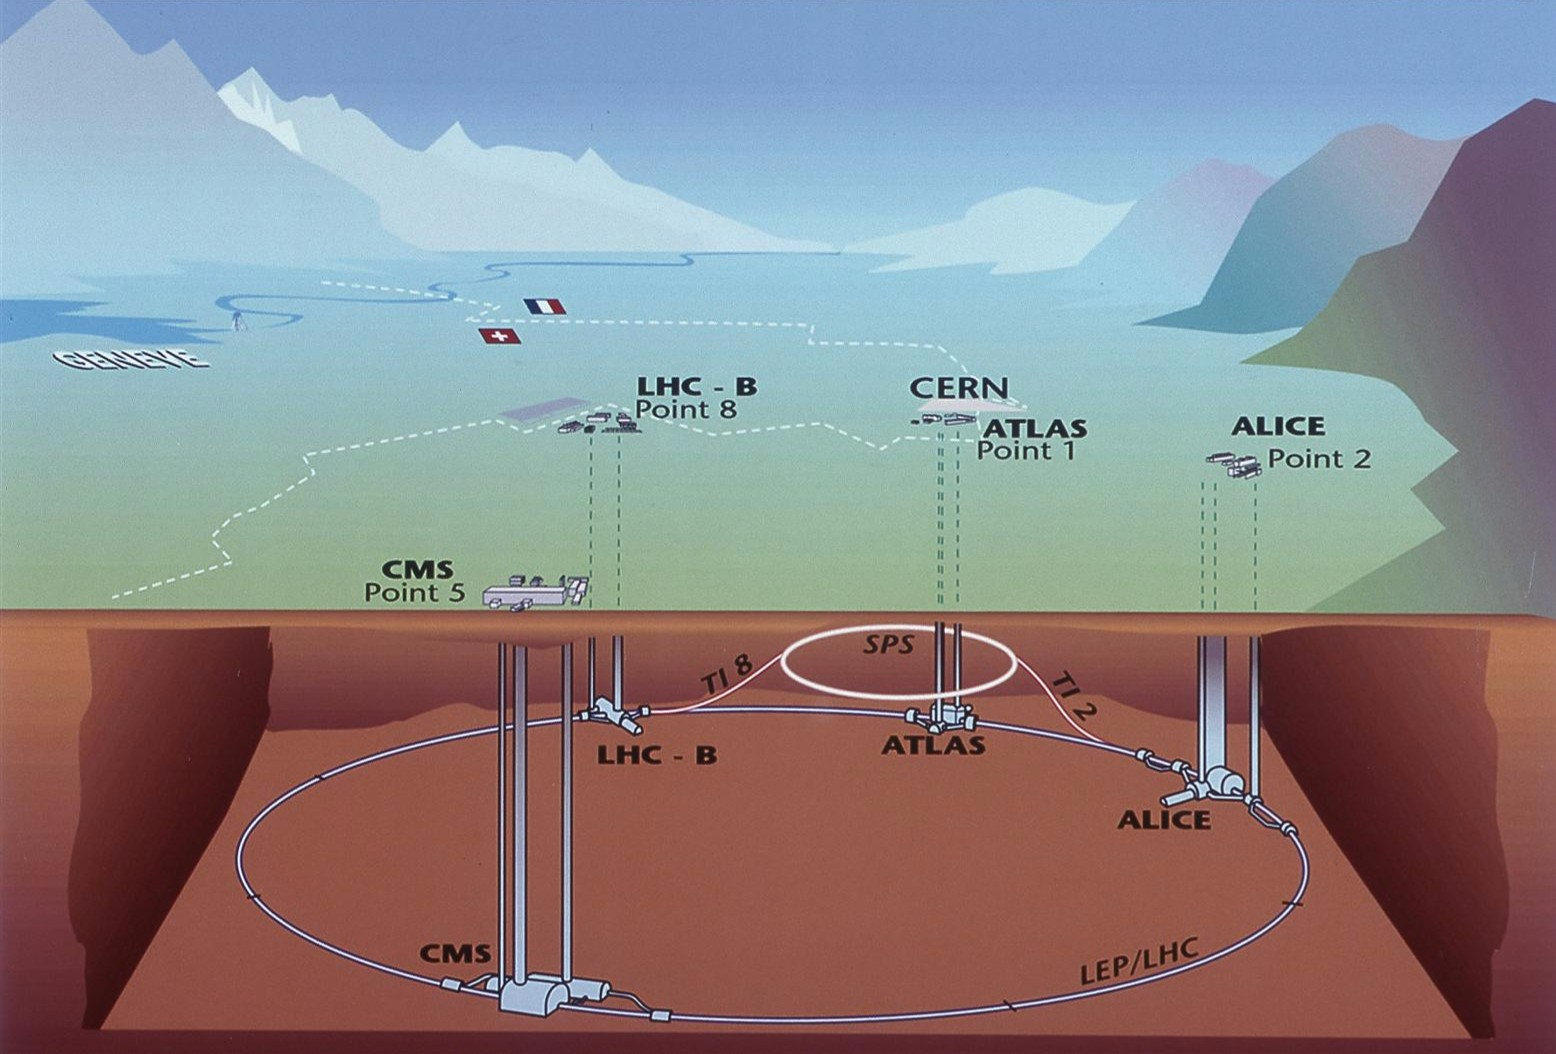
\includegraphics[width=\fullfig]{figures/cern_locations.jpg}
\caption{The four collision points and corresponding experiments of the \ac{LHC}. The image includes the location of the nearby city of Geneva as well as the border of France and Switzerland.}
\label{fig:cern_locations}
\end{figure}

\section{Injection Chain}
The \ac{LHC} takes advantage of the presence of previously built accelrators at \ac{CERN} to work up to the target energy in consecutive stages.
The series of accelerators that feed into the \ac{LHC} are known collectively as the injection chain, and together with the \ac{LHC} form the accelerator complex.
The full complex is illustrated in Figure~\ref{fig:accelerator_complex}, which details the complex series required to reach collisions of 13 or 14 \TeV. 

\begin{figure}[h]
\centering
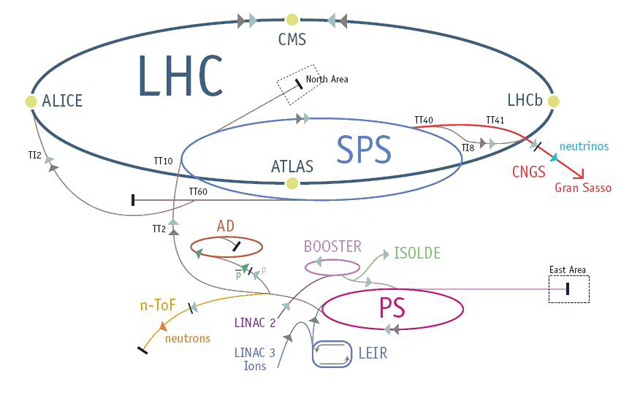
\includegraphics[width=\fullfig]{figures/accelerator_complex.jpg}
\caption{The accelerator complex that builds up to the full design energies at the \ac{LHC}. The protons are passed in order to Linac 2, the \acs{PSB}, the \acs{PS}, the \acs{SPS} and then the \ac{LHC}.}
\label{fig:accelerator_complex}
\end{figure}

Protons at the \ac{LHC} begin as hydrogen atoms in the Linac 2, a linear accelerator which replaced Linac 1 as the primary proton accelerator at CERN in 1978.
In Linac 2, the hydrogen atoms are stripped of their electrons by a strong magnetic field, and the resulting protons are accelerated up to 50 \MeV by cylindrical conductors charged by radiofrequency cavities.
The protons are then transferred to the \ac{PSB}, which uses a stack of four synchroton rings to accelerate the protons up to 1.4 \GeV.
Then the protons are injected into the \ac{PS} which again uses synchroton rings to bring the energy up to 25 \GeV.
The intermediate step between Linac 2 and the \ac{PS} is not directly necessary, as the \ac{PS} can accelerate protons starting from as low as 50 \MeV.
The inclusion of the \ac{PSB} allows the \ac{PS} to accept a higher intensity of injection and so increases the deliverable luminosity in the \ac{LHC}.
The penultimate stage of acceleration is provided by the \ac{SPS}, a large synchrotron with a 7 km circumference that was commisioned at CERN in 1976.
During this step the protons increase in energy to 450 \GeV, after which they can be directly injected into the \ac{LHC}. 


The final step is the \ac{LHC} itself, which recieves protons from the \ac{SPS} into two separate beam pipes which circulate in opposite directions.
The filling process at this steps takes approximately 4 minutes, and the subsequent acceleration to the final energy (6.5 \TeV during 2015 and up to 7 \TeV by design) takes appriximately half an hour.
At this point the protons circulate around the circumference tens of thousands of times a second and continue for up to two hours.

% ----------------------------------------

\section{Design and Parameters}

\subsection{Layout}

Many of the aspects of the \ac{LHC} design are driven by the use of the existing \ac{LEP} tunnel. 
This tunnel slopes gradually, with a 1.4\% decline, with 90\% of its length built into molasse rock which is particularly well suited to the application.
The circumference is composed of eight 2987 meter arcs and eight 528 meter straight sections which connect them; this configuration is illustrated in Figure~\ref{fig:lhc_schematic}.
The tunnel diameter is 3.7 m throughout its length. 

\begin{figure}
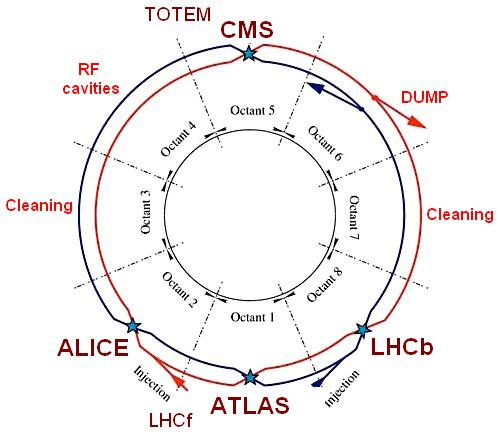
\includegraphics[width=\fullfig]{figures/lhc_schematic.jpg}
\caption{A schematic of the layout of the \ac{LHC}, not to scale. The arched and straight sections are illustrated at the bottom of the schematic, and all four crossing sites are indicated with their respective experiments.}
\label{fig:lhc_schematic}
\end{figure}

The design energy is directly limited by the size of this tunnel, with its radius of curvature of 2804 m. 
A significant magnetic field is required to curve the protons around that radius of curvature; the relationship is given by:

\[ p \simeq 0.3BR\]

\noindent where p is the momentum of the particle in \GeV, B is the magnetic field in Tesla, and R is the radius of curvature in meters. 
From the target design energy of 14 \TeV, or 7 \TeV of momentum for protons in each beam, the required magnetic field is 8.33 Tesla.
This is too large a field strength to be practical with iron electromagnets, because of the enormous power required and the resulting requirements for cooling.
Because of these constraints, the \ac{LHC} uses superconducting magnets which can maintain that field strength with signficantly less power comsumption.

\subsection{Magnets}

Specifically the magnets chosen were Niobium and Titanium (NbTi) which allow for field strengths as high as 10 Tesla when cooled down to 1.9 K.
Reach 1.9 K for all of the magnetis requires superfluid helium and a large cryogenic system along the entire length of the tunnel.
During normal operation, the \ac{LHC} uses 120 tonnes of helium within the magnetics, and the entire system is cooled by eight cryogenic helium refrigerators.
The temperature increase that occurs during transit from the refrigerator along the beam necessitates that the refrigerators cool the helium down to 1.8 K.

In all there are approximately 8000 superconducting magnets distributed around the \ac{LHC}.
The 1232 bending magnets, which keep the protons curving along the length of the beam, are twin bore cryodipoles, which allow both proton beams to be accomodated by one magnet and all of the associated cooling structure.
Figure~\ref{fig:dipole_magnet} shows the cross section of the design for these dipoles. 
The magnets are very large, 16.5 m long with a diameter of 0.57 meters and a total weight of 28 tonnes. 
They are slightly curved, with an angle of 5.1 mrad, in order to carefully match the beam path.
The twin bore accomodates both magnets inside the two 5 cm diameter holes which are surrounded by the superconducting coils.
The coils require 12 kA of current in order to produce the required magnetic field.
These coils are comprised of NbTi cable wound in two layers; the wire in the inner layer has a diameter of 1.065 mm while the wire in the outer layer has a diameter of 0.825 mm. 

\begin{figure}
\centering
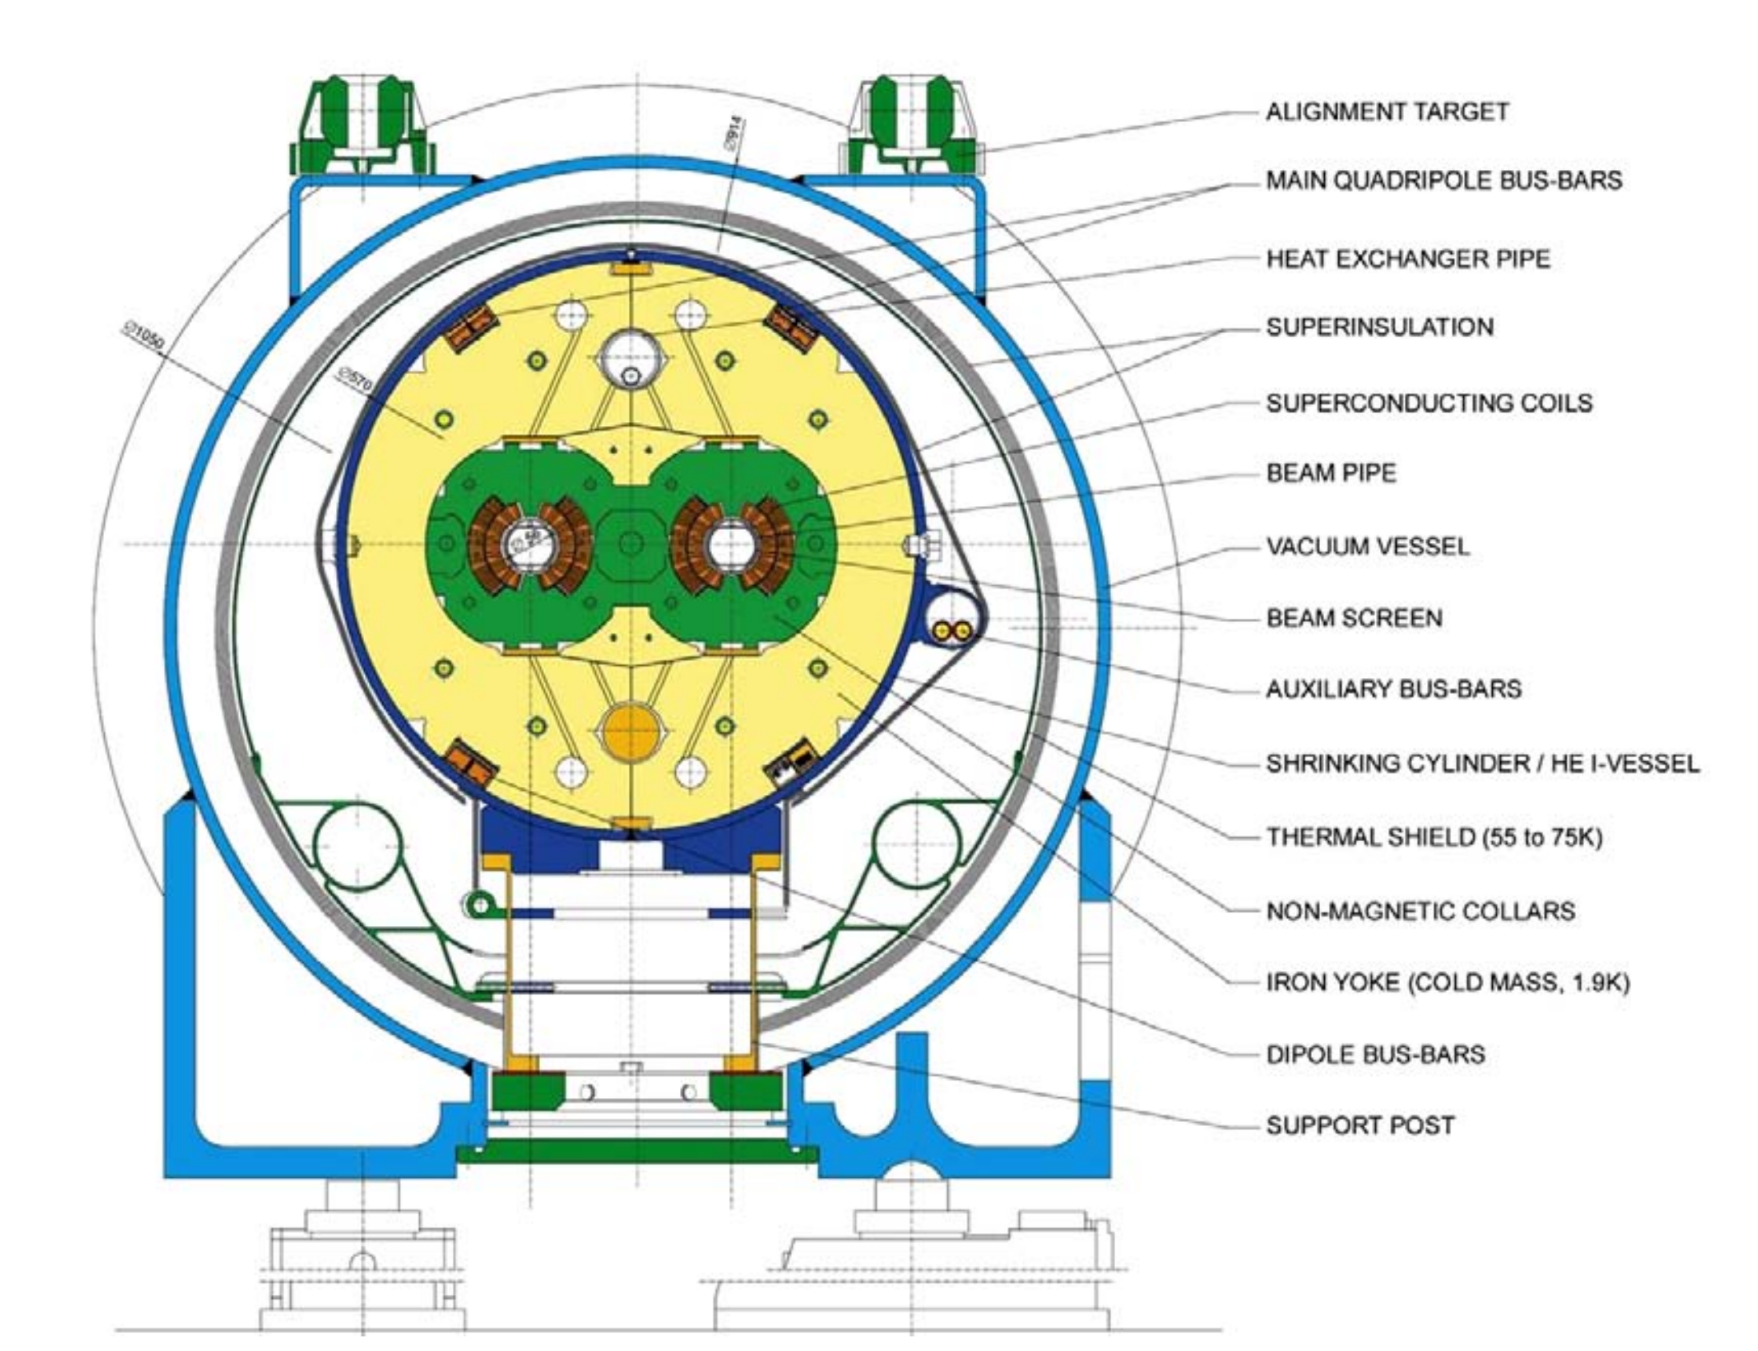
\includegraphics[width=\fullfig]{figures/dipole_magnet.png}
\caption{A cross section of the the cryodipole magnets which bend the flight path of protons around the circumference of the \ac{LHC}. The diagram includes both the superconducting coils which produce the magnetic field and the structural elements which keep the magnets precisely aligned.}
\label{fig:dipole_magnet}

\end{figure}

The large current in the wires, along with the magnetic field produced, result in forces on the magnets which would tend to push them apart with over 10,000 Newtons per meter.
Constraining the magnets requires a significant amount of structure including non-magnetic stainless steel collars. 
Both the presenece of these electromagnetic forces and the varying thermal contraction coefficient of the pieces of the magnet produce significant forces on the cold mass structure. 
The cold mass is carefully engineered to so that these stresses do not significantly alter the magnetic field shape, which must be maintained between magnets to a precision of approximately $10^{-4}$ for succesful operation.

The remaining 6800 magnets are a variety of quadrupole, sextapole, octopole, and single bore dipole magnets.
These are used to damp oscillations, correct beam trajectories, focus the beams during circulation, and to squeeze the beams before collisions.



% Talk about the beam pipe later!

% ----------------------------------------

\section{Luminosity}

% ----------------------------------------
